\chapter{Asset Allocation}
\label{chpr:ch5}
\bigskip

The goal of this chapter is to investigate wether including cryptoassets in an investment portfolio could generate profits and advantages in terms of diversification or not. This investigation has been done by working on the idea of efficient frontier and optimal allocation. In particular, the considered framework is the well known Markowitz's Portfolio Theory.

After that, the focus will move on the differences from an investment portfolio that includes multiple cryptoassets and an investment porfolio that includes bitcoin as the only cryptoasset.


\section{Markowitz's Portfolio Theory}
Harry Markowitz is highly regarded as a pioneer for his theoretical contributions to
financial economics and corporate finance. In 1990, he won a Nobel Prize for his
contributions to these fields, which he explained in his “Portfolio Selection” \citep{mark52} essay first published in
The Journal of Finance, and more extensively in his book, “Portfolio Selection: Efficient Diversification" \citep{mark59}. His studies gave rise to the ‘Modern
Portfolio Theory’ (MPT). The foundation for this theory was substantially later expanded upon by
Markowitz’ fellow Nobel Prize co-winner, William Sharpe, who is widely known for his 1964 Capital
Asset Pricing Model work on the theory of financial asset price formation.

Essentially, MPT is an investment framework where the goal is to select financial instruments in order to maximize the portfolio's expected returns with the minimun risk, that is measured by the portfolio volatility. In order to get the minimum possible volatility what comes to our help is the principle of diversification: this idea was well summarized in \citep{Fabozzi7} with the sentence \textit{"don't put all your eggs in one basket"}.

\noindent
Even if cryptoassets have higher volatility with respect to other instrument, they have almost zero correlations with the market, and thus they could increase returns without affecting much the overall portfolio volatility.


Consider now a set of $N$ financial instrument represented through a vector $S$ by which we would like to construct our investment portfolio. Let's call $w$ the vector of which element $w_i$ represent the percentage of our wealth that we invest in the instrument $S_i$.


\noindent
Consider $\mathop{\mathbb{E}}\left[ R_p  \right]$ the expected return of our portfolio: it is defined as

\begin{equation}
    \mathop{\mathbb{E}}\left[ R_p  \right] = \sum_{i=0}^{N}\mathop{\mathbb{E}}\left[ w_i R_i  \right]
\end{equation}
where $R_i$ is the return of the instrument $S_i$.

\noindent
We now define the portfolio volatility $\sigma_p$ as
\begin{equation}
    \sigma_p = \sqrt{\sigma_p^2}
\end{equation}
with
\begin{equation}
    \sigma_p^2 = \sum_{i=1}^N w_i^2 \sigma_i^2 + \sum_{i=1}^N \sum_{j=1, j\neq i}^N w_i w_j \sigma_i \sigma_j \rho_{ij}
\end{equation}
where $\sigma_i$  is the (sample) standard deviation of the periodic returns of the instrument $S_i$, and $\rho_{ij}$ is the correlation coefficient between the returns on instruments $S_i$ and $S_j$.
Finally let's call $\Sigma$ the covariance matrix of the N instruments returns $R_i$.

\noindent
Now we can define the Portfolio Frontier $\mathcal{W}^*$:

consider $\mathcal{W}$ the set of all possible portfolios, then $\mathcal{W}^*$ is the subset of $\mathcal{W}$ which contains all the portfolios $w$ that solve the following quadratic problems
\begin{equation}
    \begin{aligned}
    \min_{w \in \mathcal{W}} \quad & \frac{1}{2}w^t \Sigma w\\
    \textrm{s.t.} \quad & \mathop{\mathbb{E}}\left[ R_p  \right] = \mu\\
      & e^T w = 1    \\
    \end{aligned}
\end{equation}
for $\mu \in \left( -\inf, \inf \right)$.

The condition $e^T w = 1$ means that the portfolio is full-invested. For simplicity in this thesis we only focus on the sub-problems with the additional condition
\begin{equation}
    \begin{aligned}
    \quad & w_i > 0 & \quad & for & i = 1,...,N   \\
    \end{aligned}
\end{equation}
which does not allow investor to sell-short the instruments.

We solved this quadratic problem by using the function \textit{solve.QP} of the R \citep{R} package \textit{quadprog} \citep{quadp} which solves quadratic programming problems with the dual method of Goldfarb and Idnani (1982, 1983) (this method is based on the fact that the unconstrained minimum of the objective function can be used as a starting point for positive definite quadratic programming problems).

The outcome is the set of portfolios with the minimum volatility for every reachable returns. An horizontal parabola is obtained by plotting the return versus volatility of those portfolios. 
Let us call the points on this parabola $w_i=(\sigma_i,r_i)$. Note that due to the properties of an horizontal parabola, for every $\sigma_i$ there are two points lying on the parabola, let's say $(\sigma_i,r_j)$ and $(\sigma_i,r_k)$. 
This means that for every level of volatility one can chose between two portfolios with different returns. Of course an investor will always choose the one with highest return, which is $(\sigma_i,max(r_j,r_k))$. 
By taking these points for each possible $\sigma_i$ we got the part of the parabola which is above the horizontal axis: this is called \textit{Efficient Frontier}.


\section{Numerical results}
\label{Numerical results}

We constructed the efficient frontier using our dataset in order to check which instruments yield a positive contribute to the portfolio.
In figure \ref{front1} there are the efficient frontiers of three portfolios:
\begin{enumerate}
    \item in black the portfolio composed of the standard instruments only (no cryptoassets)
    \item in blue the portfolio composed of the standard instruments plus Bitcoin
    \item in red the portfolio composed of all the instruments of the dataset
\end{enumerate}

\begin{figure}[H]
    \centering
    \makebox[\textwidth][c]{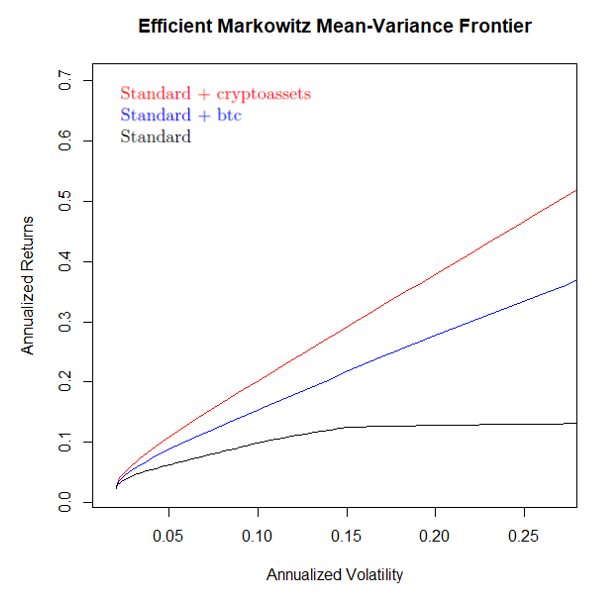
\includegraphics[width=12cm, height=12cm]{Images/chap5/frontiera_l.png}}
    \caption{Efficient frontier over the whole dataset time period}
    \label{front1}
\end{figure}
\bigskip

Here we see that each of these frontiers are different from each other. In particular the more instruments we include, the higher return we get (by fixing a target volatility). From this first analysis one could conclude just that including more instruments is in general positive. This consideration is just another way to define the diversification principle.

Something strange is that after our considerations about the correlations inside the world of cryptoassets one could expect to see almost no differences between the portfolio with just Bitcoin and the one with all the cryptoassets since it's hard to reduce the portfolio volatility by combining them.
Another important thing to say is that this asset class was born not so far and this could affects results: in general, when there is a new instrument in the market it takes some time for it to be priced at the right level and to become efficient. Just thinking about an IPO for a stock, in the first days of trading it usually move  faster than usual stocks.

For these reasons we then repeated the calculations to obtain the efficient frontier considering just the second half of the dataset time period, that means starting from the $14^{th}$ July of 2017. 

\begin{figure}[H]
    \centering
    \makebox[\textwidth][c]{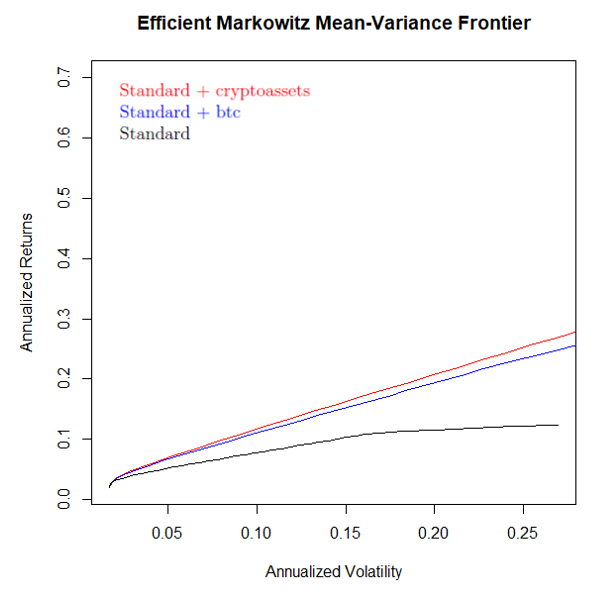
\includegraphics[width=12cm, height=12cm]{Images/chap5/frontiera_mezzo_l.png}}
    \caption{Efficient frontier over the periof from the $13^{th}$ July of 2017 to the $4^{th}$ of May of 2019}
\end{figure}
\bigskip


The black line remains almost unchanged while the red and blue ones have gone down. This happens even if the considered time window still contains the period of biggest increase of cryptoassets, which is the last part of 2017. That is because that period was characterized by a very high volatility and so it causes a lower wealth allocation in cryptoassets.

Even more important is the fact that the red and blue lines get closer with respect to the previous case. 
The distance between them is very small and we can consider them almost equals. This means that including Bitcoin or including all the top four cryptoassets by exchanged volumes makes no differences in terms of performance versus volatility.

In \autoref{chpr:ch3} we studied the correlations between cryptoassets and we have seen that, after a period where the correlations were relatively small, they go up and the p-values go down. Of course this is one of the reasons that makes the frontiers closer after the first half of the data sample: the high correlations don't allow to reduce the volatility by including different cryptoassets.
\bigskip

In the following table we report the return of the best portfolios which are the one that have the best Sharpe ratio.

\begin{table}[H]
    \centering
    \begin{tabular}{l|c|c}
         & Whole dataset & Second half \\
         \hline
         \textcolor{red}{Standard + cryptoassets} & 8.87\% & 3.59\% \\
         \textcolor{blue}{Standard + btc} & 5.87\% & 3.62\% \\
         Standard & 3.88\% & 3.05\% \\
    \end{tabular}
    \caption{Return of the best portfolio for each frontier in terms of Sharpe ratio}
    \label{tab:sharpratios}
\end{table}

The Sharpe ratio \textit{SR} is a measure of the goodness of a portfolio. It is defined as:
\begin{equation}
    SR = \frac{R_p - R_f}{\sigma_p}
\end{equation}

where $R_p$ and $\sigma_p$ are respectively the return and the volatility of the portfolio and $R_f$ is  the risk free rate. In our analysis we considered a risk free rate equal to 0 since we are doing a comparison analysis and not an absolute one: we're not interested in evaluating in this way the absolute goodness of these portfolios.

In the \autoref{tab:sharpratios} there is no new information with respect to the graphs above. We report these values just to identify a precise portfolio over each of the three frontiers. We now analyse the allocation for each of them.

\begin{table}[H]
    \centering
    \begin{tabular}{c|ccc|}
         &  \multicolumn{3}{c|}{Whole dataset} \\
         \cline{2-4}
          & \textcolor{red}{Standard + cryptoassets} & \textcolor{blue}{Standard + btc} & Standard\\
          \hline
          bric & 0.34\% & 1.13\% & 0.83\% \\
          sp500 & 4.31\% & 4.57\% & 4.35\% \\
          eurostoxx & 0.00\% & 0.00\% & 0.00\%\\
          nasdaq & 6.21\% & 6.24\% & 6.83\% \\
          bond\_europe & 0.00\% & 0.00\% & 0.00\%\\
          bond\_us & 76.14\% & 75.16\% & 70.52\\
          bond\_eur & 4.86\% & 5.69\% & 12.78\%\\
          eur & 0.00\% & 0.00\% & 0.00\%\\
          gbp & 0.00\% & 0.00\% & 0.00\%\\
          chf & 0.00\% & 0.00\% & 0.00\%\\
          jpy & 0.00\% & 0.00\% & 0.00\%\\
          gold & 0.00\% & 0.00\% & 0.52\%\\
          wti & 1.87\% & 1.44\% & 1.26\%\\
          grain & 0.00\% & 0.00\% & 0.00\%\\
          metal & 2.28\% & 2.84\% & 2.91\%\\
          btc & 1.19\% & 2.93\% & \\
          eth & 1.78\% & &\\
          ltc & 0.00\% & &\\
          xrp & 1.03\% & &\\
    \end{tabular}
    \caption{Allocations for the best Sharpe ratio portfolios considering the whole dataset}
    \label{tab:allocationsharpe}
\end{table}

In \autoref{tab:allocationsharpe} the most significant differences among the portfolios are the increasing weight of bond\_eur and the decreasing weight of bond\_us in removing the cryptoassets. Another important factor is of course the weight assigned to the cryptoassets: it goes from 2.93\% in the \textcolor{blue}{Standard + btc} case to a total of 4.00\% in the \textcolor{red}{Standard + cryptoassets} case while the weight of btc goes from 2.93\% to 1.19\%. From this table it seems there is a difference in terms of performance and allocation if we include in our investable universe all the cryptoassets or just Bitcoin.

\begin{table}[H]
    \centering
    \begin{tabular}{c|ccc|}
         &  \multicolumn{3}{c|}{Second half} \\
         \cline{2-4}
          & \textcolor{red}{Standard + cryptoassets} & \textcolor{blue}{Standard + btc} & Standard \\
          \hline
          bric & 0.00\% & 0.00\% & 0.00\%\\
          sp500 & 4.35\% & 3.37\% & 3.90\%\\
          eurostoxx & 0.00\% & 0.00\% & 0.00\%\\
          nasdaq & 0.69\% & 1.94\% & 1.58\%\\
          bond\_europe & 0.00\% & 0.00\% & 0.00\%\\
          bond\_us & 35.99\% & 39.03\% & 35.17\%\\
          bond\_eur & 55.32\% & 51.87\% & 56.77\%\\
          eur & 0.00\% & 0.00\% & 0.00\%\\
          gbp & 0.00\% & 0.00\% & 0.00\%\\
          chf & 0.00\% & 0.00\% & 0.00\%\\
          jpy & 0.85\% & 0.66\% & 0.76\%\\
          gold & 0.00\% & 0.00\% & 0.00\%\\
          wti & 1.86\% & 2.11\% & 1.82\%\\
          grain & 0.00\% & 0.00\% & 0.00\%\\
          metal & 0.00\% & 0.00\% & 0.00\%\\
          btc & 0.63\% & 1.02\% &\\
          eth & 0.00\% & &\\
          ltc & 0.00\% & &\\
          xrp & 0.30\% & & \\
    \end{tabular}
    \caption{Allocations for the best Sharpe ratio portfolios considering the second half of the dataset}
    \label{tab:allocationsharpe_2}
\end{table}

In \autoref{tab:allocationsharpe_2} we get in general a smaller allocation in cryptoassets even if in the second half of the dataset the peak reached in 2017 by the cryptoassets in general is still included. One more interesting fact is that the total allocation in cryptoassets remains at about 1\% in both the case of \textcolor{blue}{Standard + btc} and \textcolor{red}{Standard + cryptoassets}.
Moreover, the frontiers of these 2 cases are so closed that the difference may not justify the addition of one instrument in the portfolio.

\section{Allocation in time}
After these studies it is relevant to analyse how the allocation changes in time.

We considered a rolling time window of 2 years on which we calculated the optimal allocation in terms of Sharpe ratio.

\begin{table}[H]
    \centering
    \resizebox{\textwidth}{!}{\begin{tabular}{c c}
    \begin{minipage}{.5\textwidth}
      \includegraphics[height=60mm, width=76mm]{Images/chap5/"roll_all_cry".png}
    \end{minipage}
    &  
    \begin{minipage}{.5\textwidth}
      \includegraphics[height=60mm, width=76mm]{Images/chap5/"roll_btc_cry".png}
    \end{minipage}\\
    \end{tabular}}
    \captionof{figure}{Optimal allocation over a rolling time window of 2 years}
    \label{tab:my_label}
\end{table}

The figure on the left represents the portfolio that contains, along with the standard instruments, also btc, ltc, eth and xrp while the one on the right includes just standard instruments and bitcoin. Allocation of standard instruments remains almost unchanged in both cases.\\
It's interesting to observe that by removing xrp, ltc and eth from the portfolio we can say that their allocation is moved completely to btc. This fact confirms what we've seen in section \ref{Numerical results}: adding cryptoassets different from btc yield no extra return and it doesn't change the portfolio allocation in standard instruments.

It is also interesting to observe that the relative allocation of standard instruments doesn't change that much by including or not cryptoassets.
\begin{table}[H]
    \centering
    \resizebox{\textwidth}{!}{\begin{tabular}{c c}
    \begin{minipage}{.5\textwidth}
      \includegraphics[height=60mm, width=76mm]{Images/chap5/"roll_all_other".png}
    \end{minipage}
    &  
    \begin{minipage}{.5\textwidth}
      \includegraphics[height=60mm, width=76mm]{Images/chap5/"roll_no_other".png}
    \end{minipage}\\
    \end{tabular}}
    \captionof{figure}{Optimal allocation over a rolling time window of 2 years with and without cryptoassets}
    \label{tab:my_label}
\end{table}

This result suggests that cryptoassets don't affect correlations between other asset classes, meaning that one can consider them as a new uncorrelated asset class.